\documentclass[10pt,a4paper]{ctexart}
\usepackage[margin=2cm]{geometry}
\usepackage{graphicx}
\usepackage{hyperref}
\usepackage{amsmath}    % 提供方程环境
\usepackage{physics}    % 简化向量、微分算子语法
\newcommand{\myspace}[1]{\par\vspace{#1\baselineskip}} %自定义空一行
\usepackage{fancyhdr}
\usepackage{float} % 强制图片位置
\usepackage{zhnumber} % 中文数字
\pagestyle{fancy}
\fancyhf{}  % 清除所有页眉页脚
\fancyfoot[C]{\thepage}  % 在页脚中央设置页码
\renewcommand{\headrulewidth}{0pt}  % 去掉页眉横线
\renewcommand{\footrulewidth}{0pt}  % 去掉页脚横线

\usepackage{hyperref}
\hypersetup{
    colorlinks=true,
    linkcolor=blue,
    filecolor=magenta,      
    urlcolor=cyan,
    pdftitle={Overleaf Example},
    pdfpagemode=FullScreen,
    }

\usepackage{titlesec}

% 重新定义section格式
\titleformat{\section}
  {\normalfont\Large\bfseries}
  {\chinese{section}、}
  {0pt}
  {}

% 给出常用字号的自定义指令
\newcommand{\chuhao}{\fontsize{42pt}{48pt}\selectfont}
\newcommand{\xiaochu}{\fontsize{36pt}{42pt}\selectfont}
\newcommand{\xiaoer}{\fontsize{18pt}{21.6pt}\selectfont}
\newcommand{\sanhao}{\fontsize{16pt}{20pt}\selectfont}
\newcommand{\xiaosan}{\fontsize{15pt}{18pt}\selectfont}
\newcommand{\sihao}{\fontsize{14pt}{18pt}\selectfont}
\newcommand{\xiaosi}{\fontsize{12pt}{16pt}\selectfont}
\newcommand{\wuhao}{\fontsize{10.5pt}{12.6pt}\selectfont}

% 定义中文数字转换
\titleformat{\section}
  {\normalfont\Large\bfseries}
  {\zhnum{section}、}  % 使用\zhnum而不是\chinese
  {0pt}
  {}

% 标题设置
\title{\xiaochu\textbf{物理实验报告}}
\author{}
\date{}

\begin{document}

\vspace*{36pt} % 顶部空白

% 居中填写区域
\begin{center}
    
\includegraphics[width = 9cm]{figure/head.png}
    
    \xiaochu\textbf{物理实验报告}
    % 预留空白区域
    \vspace{13pt}
    \vspace{13pt}
    \vspace{13pt}
    \vspace{13pt}
    
    \sanhao\textbf{实验名称：\underline{\makebox[10cm]{ 光电效应测定普朗克常量}}} \\[10pt]
    \sanhao\textbf{实验桌号：\underline{\makebox[10cm]{ 4}}} \\[10pt]
    \sanhao\textbf{指导教师：\underline{\makebox[10cm]{ 史明 }}} \\[30pt]
    
    % 预留空白区域
    \myspace{6}
    
   \sihao\textbf{班级：\underline{\makebox[6cm]{}}} \\[10pt]
    \sihao\textbf{姓名：\underline{\makebox[6cm]{}}} \\[10pt]
    \sihao\textbf{学号：\underline{\makebox[6cm]{}}} \\[30pt]
    
   \sihao\textbf{实验日期: 
   \underline{\makebox[0.8cm]{2025}}  年 
   \underline{\makebox[0.4cm]{10}}月
   \underline{\makebox[0.4cm]{15}}日  
   星期\underline{\makebox[0.6cm]{三}}上午}
    
    \vspace{18pt}
    \sihao 浙江大学物理实验教学中心
    
\end{center}

\newpage

\section{预习报告}

    \subsection{实验综述}
    
    \xiaosi （自述实验现象、实验原理和实验方法，不超过300字，5分）
    
    光电效应是光照射金属表面时电子逸出的现象。
实验现象表明：存在截止频率$\nu_0$，低于此频率无光电流；光电子的最大初动能与光强无关。
依据爱因斯坦光电效应方程$h\nu = \frac{1}{2}mv_m^2 + W$ 和$eU_0=\frac{1}{2}mv^2_m$ 有$U_0=\frac{h}{e} \nu-\frac{W}{e}$，其中$W$为逸出功。
实验通过测量不同频率$\nu$单色光照射下的遏止电压$U_0$，验证$U_0-\nu$的线性关系：$U_0 = \frac{h}{e}\nu - \frac{W}{e}$。
使用汞灯光源配合滤光片获得单色光，调节反向电压使光电流为零，此时电压即为$U_0$。
绘制$U_0-\nu$曲线，其斜率$k = h/e$，可计算普朗克常量$h = ke$。

此外，通过测量光电管电压和电流可绘制光电管的伏安特性曲线，测量光源距离、光阑孔径和饱和光电流可以验证饱和光电流与光强的正比关系。
    \myspace{2}
    
    
    \subsection{实验重点}
    
    \xiaosi（简述本实验的学习重点，不超过100字，3分）
    
1. 精确测量不同频率光对应的遏止电压$U_0$ 
 
2. 准确绘制$U_0-\nu$图像并计算斜率，通过斜率$k$计算普朗克常量$h = ke$ 

3. 掌握消除暗电流和本底电流影响的方法
    \myspace{2}
    
    \subsection{实验难点}
    
    \xiaosi（简述本实验的实现难点，不超过100字，2分）

1. 遏止电压$U_0$的准确判定：实际光电流为零点难以确定 

2. 暗电流和反向电流的干扰，需使用方法减少其影响和干扰 

3. 杂散光影响测量精度 

4. 光电管疲劳效应引起的灵敏度变化
\myspace{2}
\section{原始数据}

    \xiaosi （将有老师签名的“自备数据记录草稿纸”的扫描或手机拍摄图粘贴在下方，20分）
\begin{figure}[H]
    \centering
    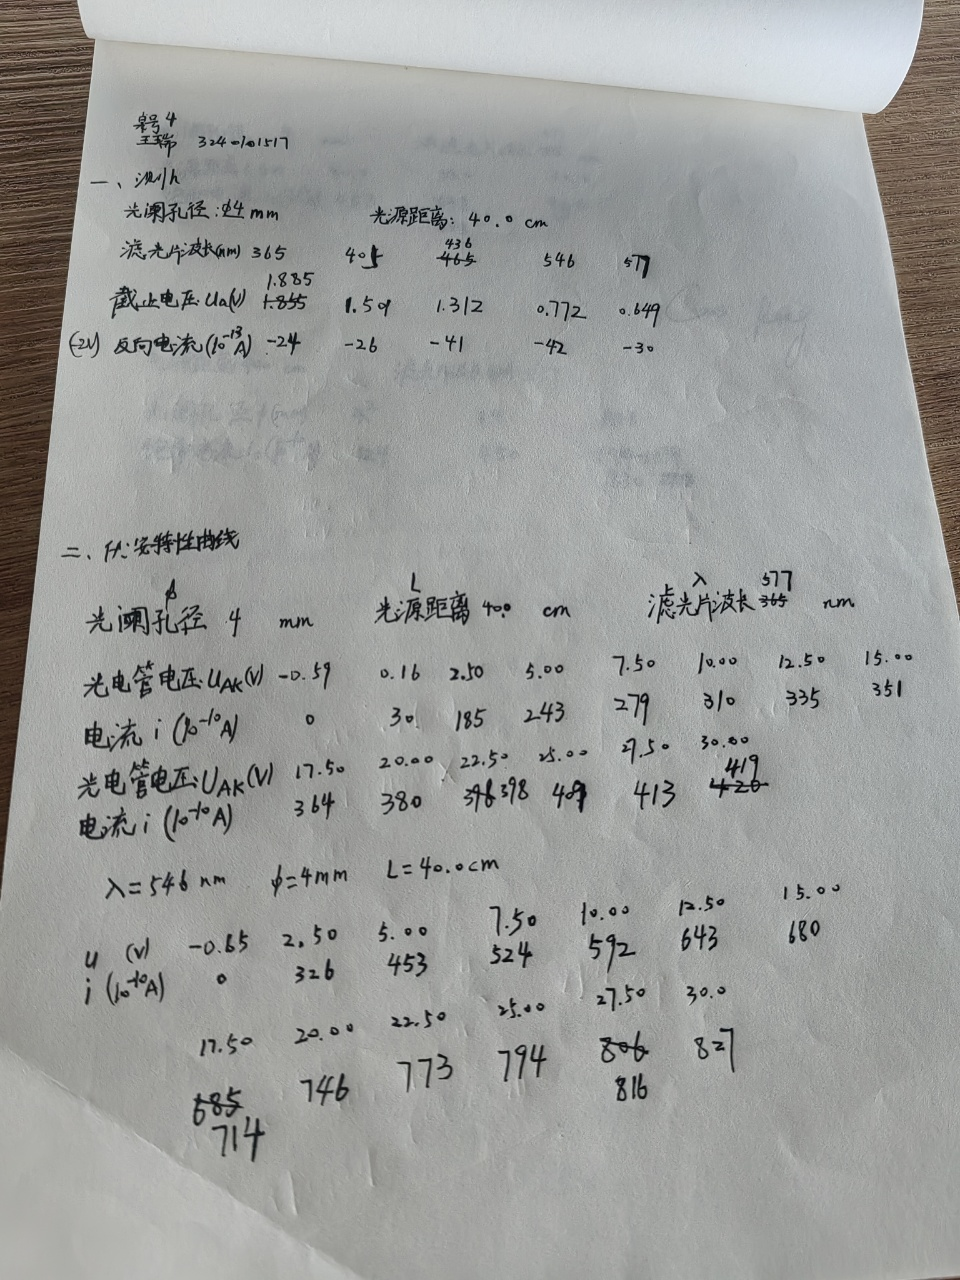
\includegraphics[width=0.9\textwidth]{figure/raw_1.jpg}
    \caption{数据记录草稿纸1}
\end{figure}
\begin{figure}[H]
    \centering
    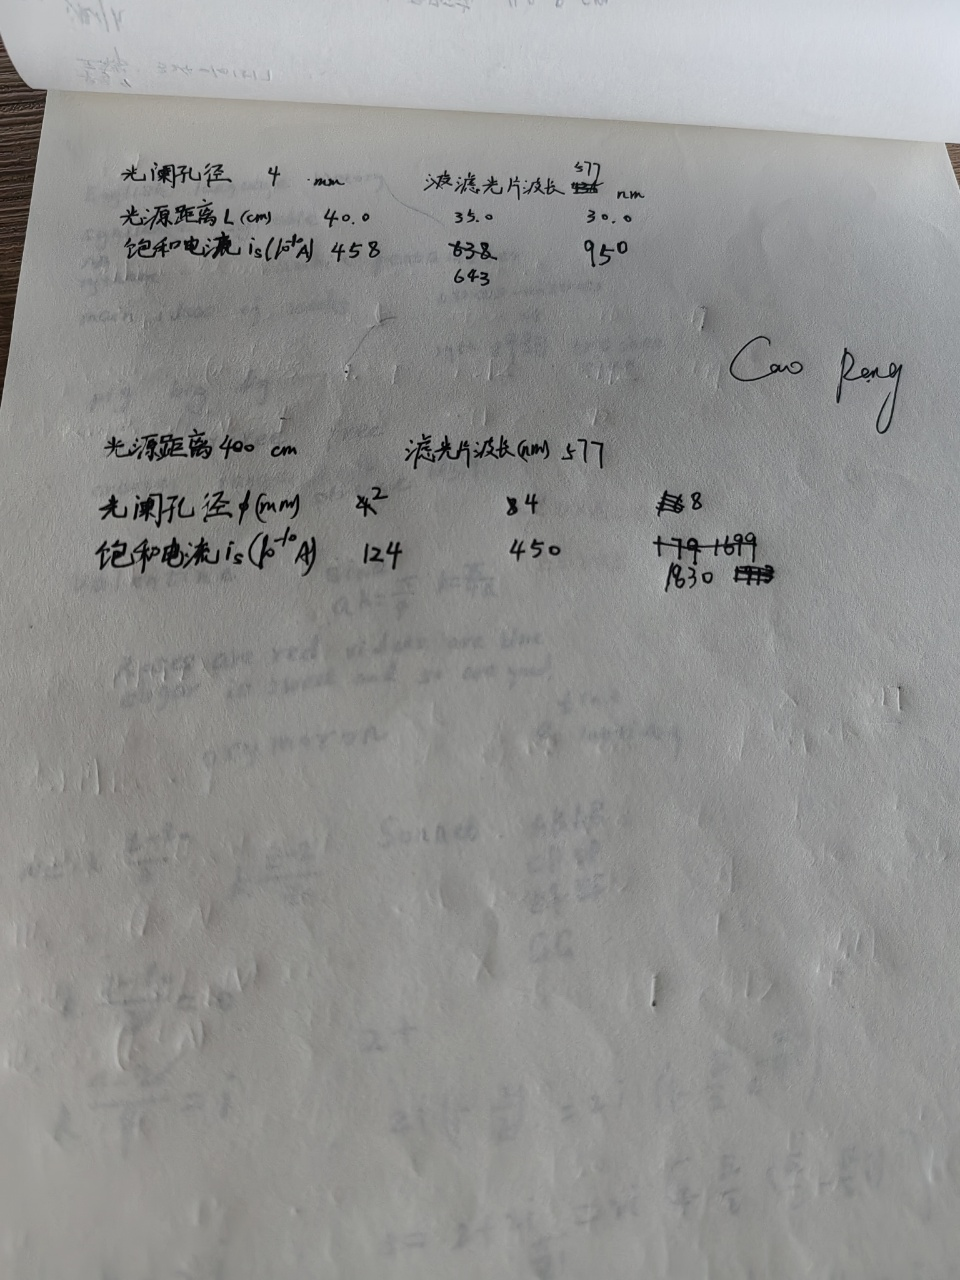
\includegraphics[width=0.9\textwidth]{figure/raw_2.jpg}
    \caption{数据记录草稿纸2}
\end{figure}
\section{结果与分析}

    \subsection{数据处理与结果}
    \xiaosi （列出数据表格、选择数据处理方法、给定测量或计算结果，30分）
\subsubsection{测量普朗克常量}
实验使用FB807 型光电效应(普朗克常数)测定仪，测量不同频率单色光对应的遏止电压$U_a$，
光阑孔径$\phi$设为4mm，光源距离L设为40.0cm，
数据如下表所示（注截止电压测得负值，此处全部取绝对值）：
\begin{table}[H]
\begin{tabular}{|l|l|l|}
\hline
滤光片波长$\lambda$（nm） & 截止电压$U_a$（V） & 反向电流I（$10^{-13}$A） \\ \hline
365                & 1.885         & -24                \\ \hline
405                & 1.501         & -26                \\ \hline
436                & 1.312         & -41                \\ \hline
546                & 0.772         & -42                \\ \hline
577                & 0.649         & -30                \\ \hline
\end{tabular}
\end{table}

根据实验数据拟合$U_a-\nu$图像如下：
\begin{figure}[H]
    \centering
    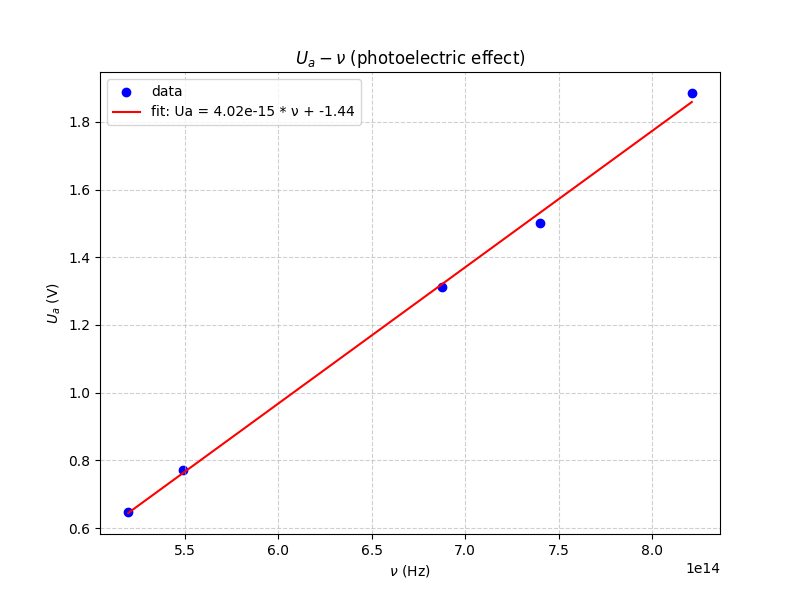
\includegraphics[width=0.7\textwidth]{figure/line.png}
    \caption{$U_a-\nu$图像拟合}
\end{figure}

使用最小二乘法拟合 $U_a - \nu$ 直线：$U_a = k \nu + b$，结果如下：

\begin{enumerate}
    \item \textbf{标准偏差}：
    最小二乘法拟合中，斜率 $k$ 和截距 $b$ 的标准偏差计算如下：
    \begin{align*}
    \sigma_k &= \sqrt{\frac{\sum_{i=1}^n (y_i - \hat{y}_i)^2}{(n-2) \sum_{i=1}^n (x_i - \bar{x})^2}} \\
    \sigma_b &= \sigma_k \sqrt{\frac{\sum_{i=1}^n x_i^2}{n}}
    \end{align*}
    其中 $n=5$ 为数据点数，$\bar{x} = 6.640 \times 10^{14}$ Hz 为频率平均值。
    
    计算结果：
    
\begin{align*}
    \sigma_k &= 9.93 \times 10^{-17}  \text{V·s} \\
    \sigma_b &= 0.067  \text{V}
    \end{align*}
    因此拟合结果为：
    $$     k = (4.021 \pm 0.099) \times 10^{-15}  \text{V·s}, \quad b = (-1.444 \pm 0.067)  \text{V}, \quad R^2 = 0.998     $$
    
    \item \textbf{普朗克常量 $h$}：
    $$     h = k e = (4.021 \times 10^{-15}) \times (1.602 \times 10^{-19}) = 6.442 \times 10^{-34}  \text{J·s}     $$
    不确定度：$u_h = e \cdot \sigma_k = 1.59 \times 10^{-35}$ J·s
    
    最终结果：
    $$     h = (6.44 \pm 0.16) \times 10^{-34}  \text{J·s}, \quad u_r = 2.48\%     $$
    与公认值比较，相对误差 $E = \dfrac{|6.44 - 6.626|}{6.626} \times 100\% = 2.81\%$。
    
    \item \textbf{功函数 $W$}：
    $$     W = |b| e = 1.444 \times 1.602 \times 10^{-19} = 2.313 \times 10^{-19}  \text{J}     $$
    不确定度：$u_W = \sigma_b \cdot e = 1.07 \times 10^{-20}$ J
    
    最终结果：
    $$     W = (2.31 \pm 0.11) \times 10^{-19}  \text{J}     $$
    
    \item \textbf{红限频率 $\nu_0$}：
    $$     \nu_0 = -\frac{b}{k} = \frac{1.444}{4.021 \times 10^{-15}} = 3.590 \times 10^{14}  \text{Hz}     $$
    不确定度：
    
\begin{align*}
    u_{\nu_0} &= \nu_0 \sqrt{ \left( \frac{\sigma_b}{b} \right)^2 + \left( \frac{\sigma_k}{k} \right)^2 } \\
    &= 1.885 \times 10^{13}  \text{Hz} \approx 1.88 \times 10^{13}  \text{Hz}
    \end{align*}
    最终结果：
    $$     \nu_0 = (3.59 \pm 0.19) \times 10^{14}  \text{Hz}     $$
\end{enumerate}
\myspace{2}
\subsubsection{绘制伏安特性曲线}
使用FB807 型光电效应(普朗克常数)测定仪，测量不同频率单色光对应的电压$U_{AK}$和电流I，光阑孔径$\phi$设为4mm，光源距离L设为40.0cm。滤光片波长分别设为：577nm和546nm，

577nm波长对应原始数据：
\begin{table}[H]
\begin{tabular}{|l|l|l|l|l|l|l|l|l|l|l|l|l|l|}
\hline
光电管电压U(V)      & -0.59 & 2.50 & 5.00 & 7.50 & 10.00 & 12.50 & 15.00 & 17.50 & 20.00 & 22.50 & 25.00 & 27.50 & 30.00 \\ \hline
光电流I($10^{-10}$ A) & 0     & 185  & 243  & 279  & 310   & 335   & 351   & 364   & 380   & 398   & 409   & 413   & 419   \\ \hline
\end{tabular}
\end{table}

546nm波长对应原始数据：
\begin{table}[H]
\begin{tabular}{|l|l|l|l|l|l|l|l|l|l|l|l|l|l|}
\hline
光电管电压U(V)      & -0.65 & 2.50 & 5.00 & 7.50 & 10.00 & 12.50 & 15.00 & 17.50 & 20.00 & 22.50 & 25.00 & 27.50 & 30.00 \\ \hline
光电流I($10^{-10}$ A) & 0     & 326  & 453  & 524  & 592   & 643   & 680   & 714   & 746   & 773   & 794   & 816   & 827   \\ \hline
\end{tabular}
\end{table}
根据数据绘制的伏安特性曲线如图：
\begin{figure}[H]
    \centering
    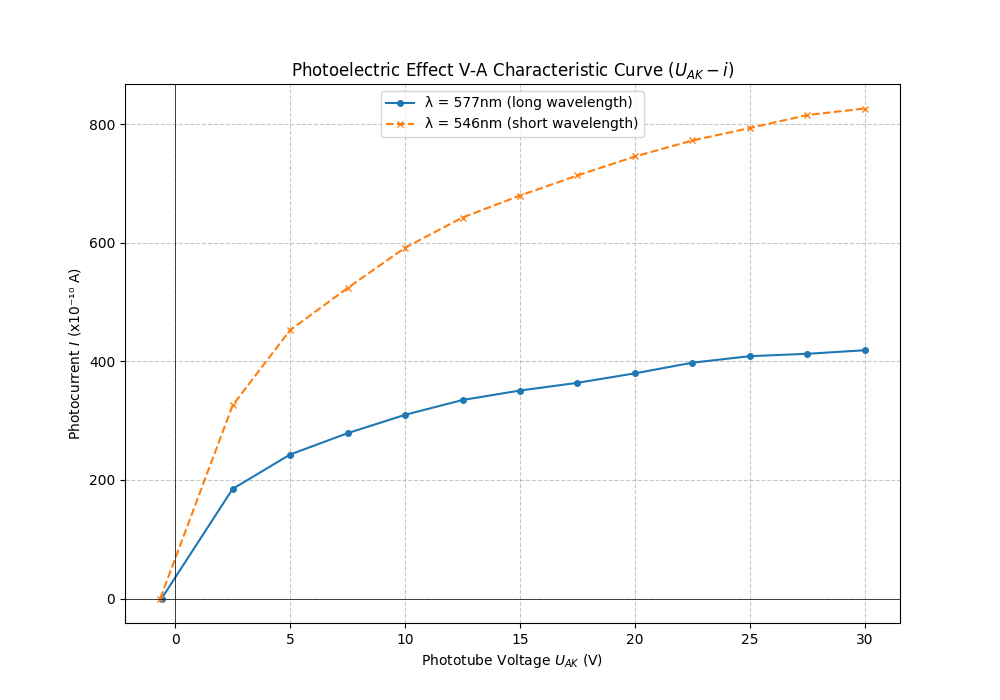
\includegraphics[width=0.9\textwidth]{figure/UI_image.png}
    \caption{伏安特性曲线}
\end{figure}

\subsubsection{验证饱和光电流与光强的关系}
理论上饱和光电流$I_s$与光强$I$成正比。
实验中通过调节光源距离L和光阑孔径$\phi$来改变光强，测量对应的饱和光电流$I_s$。
光阑孔径$\phi$设为4mm，滤光片波长设为577nm时控制光源距离L，测得数据如下：
\begin{table}[H]
\begin{tabular}{|l|l|l|l|}
\hline
光源距离L(cm) & 30.0 & 35.0 & 40.0 \\ \hline
饱和光电流$I_s$($10^{-10}$ A) & 950 & 643 & 458 \\ \hline
\end{tabular}
\end{table}
根据数据绘制的$I_s - \frac{1}{L^2}$图像如下：
\begin{figure}[H]
    \centering
    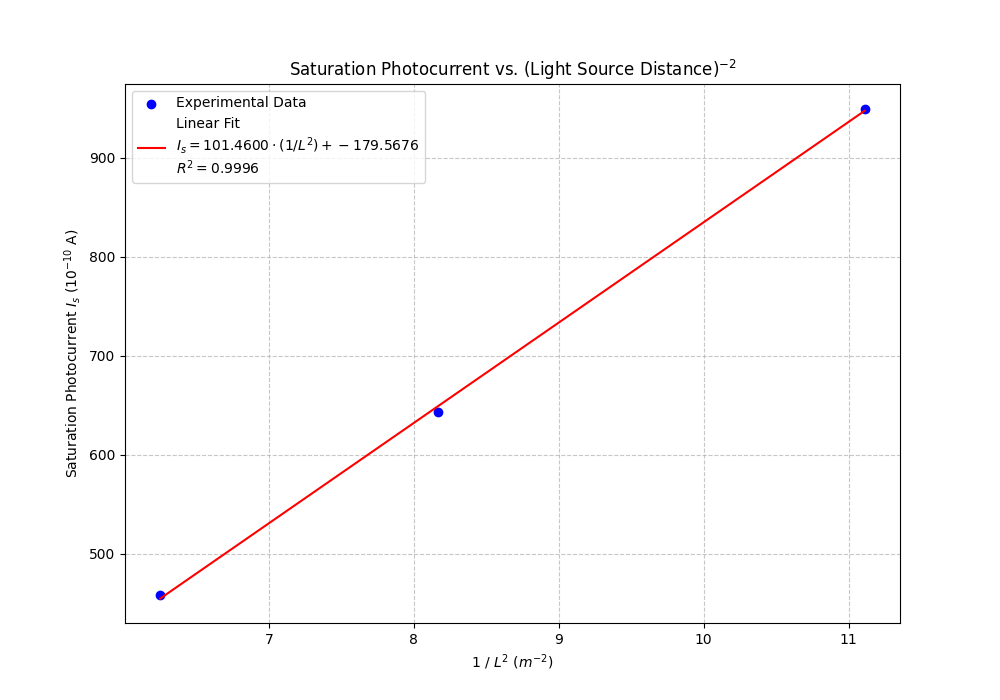
\includegraphics[width=0.7\textwidth]{figure/LI_image.png}
    \caption{$I_s - \frac{1}{L^2}$图像}
\end{figure}
拟合方程为$I_s = k \frac{1}{L^2} + b$，结果如下：
$$ k = 101.4600 \text{m}^2 \text{A}, \quad b = -179.5676  \text{A}, \quad R^2 = 0.9996 $$

光源距离L设为40.0cm，滤光片波长设为577nm时控制光阑孔径$\phi$，测得数据如下：
\begin{table}[H]
\begin{tabular}{|l|l|l|l|}
\hline
光阑孔径$\phi$(mm) & 2 & 4 & 8 \\ \hline
饱和光电流$I_s$($10^{-10}$ A) & 124 & 450 & 1830 \\ \hline
\end{tabular}
\end{table}
根据数据绘制的$I_s - \phi^2$图像如下：
\begin{figure}[H]
    \centering
    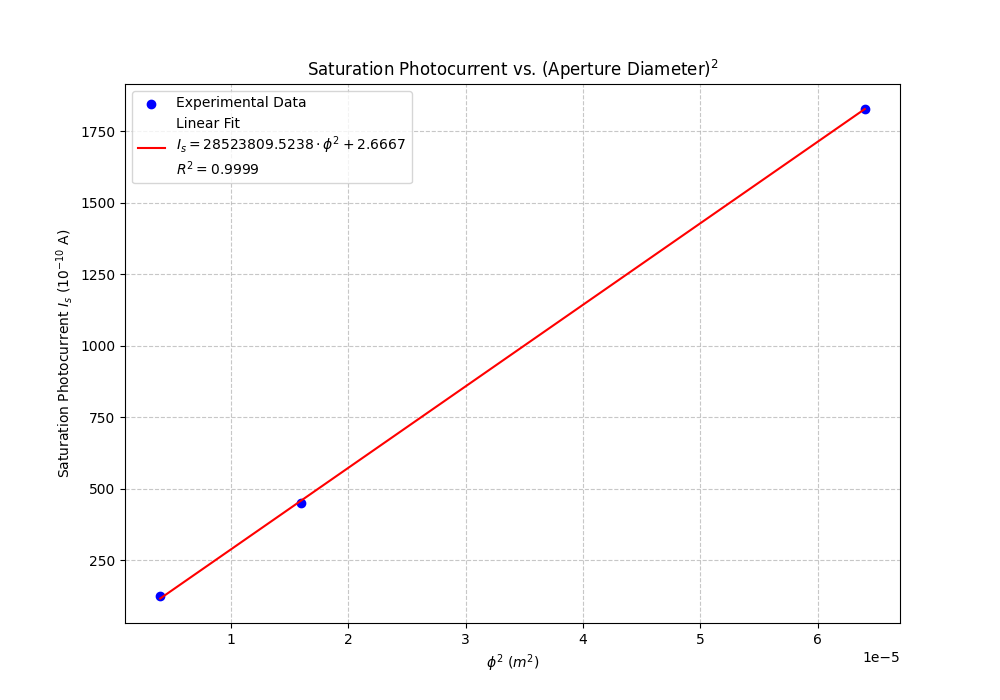
\includegraphics[width=0.7\textwidth]{figure/phiI_image.png}
    \caption{$I_s - \phi^2$图像}
\end{figure}
拟合方程为$I_s = k \phi^2 + b$，结果如下：
$$ k = 2.8524 \times 10^7 \text{m}^{-2} \text{A}, \quad b = 2.6667  \text{A}, \quad R^2 = 0.9999 $$
可以看到两个实验结果均表明饱和光电流$I_s$与光强成正比关系，验证了理论预期。
    \subsection{误差分析}
    \xiaosi （运用测量误差、相对误差、不确定度等分析实验结果，20分）
    
本实验的误差主要来源于以下几个方面：
    
\begin{enumerate}
        \item \textbf{系统误差}：
        \begin{itemize}
            \item 暗电流和本底电流：光电管在没有光照时存在暗电流，环境杂散光引起本底电流，影响截止电压的测量
            \item 滤光片的单色性：滤光片有一定的带宽，导致频率不准确
            \item 仪器零点漂移：电压表和电流表的零点可能存在漂移
        \end{itemize}
        \item \textbf{随机误差}：
        
\begin{itemize}
            \item 读数误差：电压和电流的读数存在视差和估读误差
            \item 调节误差：调节电压使电流为零时存在判断误差
            \item 环境因素：温度、湿度变化影响仪器稳定性
        \end{itemize}
        \item \textbf{其他因素}：
        
\begin{itemize}
            \item 光电管的疲劳效应：长时间光照导致灵敏度下降
            \item 光源的不稳定性：汞灯光强随时间变化
            \item 光路调整：光源与光电管之间的距离和角度调整不精确
        \end{itemize}
    \end{enumerate}
    \subsection{实验探讨}
    \xiaosi （对实验内容、现象和过程的小结，不超过100字，10分）

本实验通过测量不同频率单色光的截止电压，验证了光电效应方程中截止电压与频率的线性关系，并成功计算出普朗克常量$h$，与公认值较为接近。
同时，通过伏安特性曲线验证了饱和光电流的存在，并验证了饱和光电流与光强的正比关系。
通过本实验，加深了对光电效应现象的理解，掌握了实验仪器的使用和数据处理方法。
\section{思考题}

    \xiaosi （解答教材或讲义或老师布置的思考题，10分）

    \subsection{爱因斯坦方程表达哪些主要内容？其物理意义是什么？}

    爱因斯坦光电效应方程为：$h\nu = \frac{1}{2}mv_m^2 + W$。主要内容包括：
    
\begin{enumerate}
        \item 光照射金属时，电子吸收一个光子的能量$h\nu$
        \item 该能量一部分用于克服逸出功$W$，另一部分转化为光电子的动能
        \item 光电子的最大初动能$\frac{1}{2}mv_m^2$与光频率$\nu$成正比，与光强无关
        \item 只有当光子能量$h\nu$大于逸出功$W$时，才能发生光电效应
    \end{enumerate}
    物理意义：揭示了光的粒子性，解释了经典电磁理论无法解释的光电效应现象。

    \subsection{除采用本实验的测试方法外，你还能提出何种实验方案来测试普朗克常量？}
  除本实验方法外，还可以采用以下方法：
    
\begin{enumerate}
        \item \textbf{氢原子光谱法}：通过测量氢原子光谱线的波长，根据巴尔末公式计算里德伯常数，进而得到普朗克常量
        \item \textbf{X射线连续谱短波限法}：测量X射线连续谱的短波限$\lambda_0$与加速电压$U$的关系，利用$eU = h c / \lambda_0$计算$h$
        \item \textbf{发光二极管（LED）法}：测量不同颜色LED的开启电压$U$和发光频率$\nu$，利用$eU \approx h\nu$计算$h$
    \end{enumerate}
    \subsection{什么是逸出功，从作图中能否得到此金属的逸出功？}
      逸出功是指电子从金属表面逸出所需的最小能量。
      在光电效应实验中，通过绘制截止电压$U_0$与入射光频率$\nu$的关系图，得到直线$U_0 = \frac{h}{e}\nu - \frac{W}{e}$，其中纵截距为$-\frac{W}{e}$。
      因此，逸出功$W$等于纵截距绝对值的$e$倍。所以，从图中可以得到逸出功。

\newpage

\sihao\textbf{注意事项：}
\xiaosi
\begin{enumerate}
    \item 用PDF格式上传“实验报告”，文件名：学生姓名+学号+实验名称+周次。
    \item  “实验报告”必须递交在“学在浙大”的本课程的对应实验项目的“作业”模块内。
    \item  “实验报告”成绩必须在“浙江大学物理实验教学中心网站”-“选课系统”内查询。
    \item 教学评价必须在“浙江大学物理实验教学中心网站”-“选课系统”内进行，学生必须进行教学评价，才能看到实验报告成绩，教学评价必须在本次实验结束后 3 天内进行。
\end{enumerate}

\vspace{1cm}
\xiaosi\centering \textbf{浙江大学物理实验教学中心制}

\end{document}